\documentclass{article}
\usepackage{ucs} 
\usepackage[utf8x]{inputenc} % Включаем поддержку UTF8  
\usepackage{amsmath}
\usepackage{tikz}
\usepackage{setspace}
\usepackage{amsfonts}
\usepackage{geometry}
\usepackage{quoting}
\usepackage[russian]{babel}  % Включаем пакет для поддержки русского языка  
\usepackage[a4paper, left=0.5cm, right=0.5cm, top=0cm, bottom=0cm]{geometry}
\begin{document}
\setlength{\parindent}{0pt}
\begin{Large}
    \textsf{\textbf{ЛинАл ДЗ №2}}
    
    Шамаев Александр    
\end{Large}
\vspace{1cm}

\textsf{\textbf{(1)}}

\hspace{1cm}
\begin{quote}

Составим систему уравнений:    

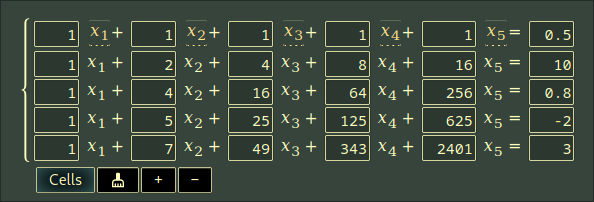
\includegraphics[width=0.5\linewidth]{2024-09-13-234400_hyprshot.png}
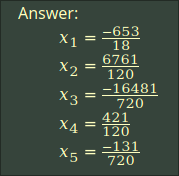
\includegraphics[width=0.2\linewidth]{image.png}

Получили функцию:
$f(x) = -\frac{653}{18}+\frac{6761}{120}x-\frac{16481}{720}x^{2}+\frac{421}{120}x^{3}-\frac{131}{720}x^{4}$

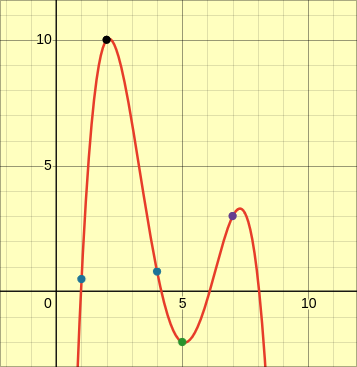
\includegraphics[width=0.5\linewidth]{2024-09-13-235821_hyprshot.png}

\end{quote}

\textsf{\textbf{(2)}}

\hspace{1cm}
\begin{quote}
Попробуем найти коэфиценты полинома третий степени, проходящего через заданные точки:

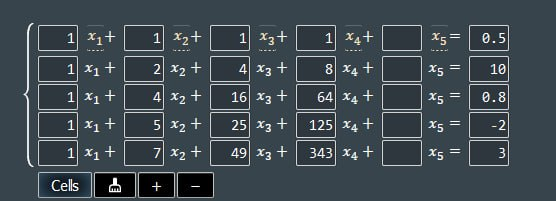
\includegraphics[width=0.5\linewidth]{photo_2024-09-15_15-44-11.jpg}

Система не имеет решений. Следовательно, полинома третей степени, проходящего через заданные точки не существует.
\end{quote}

\textsf{\textbf{(3)}}
\begin{quote}
    (a) Не выполняется третья аксиома:

    $\begin{pmatrix} a\\ b\end{pmatrix} \oplus \begin{pmatrix} c\\ d\end{pmatrix}: = \begin{pmatrix} a+c\\ b+d\end{pmatrix} = \begin{pmatrix} a \\ b \end{pmatrix} $ - Верно, если$ \begin{pmatrix} c \\ d \end{pmatrix} = \begin{pmatrix} 0 \\ 0\end{pmatrix}$, т.е. $c = d = 0$, однако, если $c = 0$, то $d = 3c + 1 = 1$. Т.е. нейтрального по сложению элемента не существует.\\
    
    (b) Не выполняется пятая аксиома:
    
     $(\alpha + \beta) \cdot \begin{pmatrix} a \\ b \end{pmatrix} = 
     \begin{pmatrix} (\alpha + \beta) \cdot a \\ b \end{pmatrix}$, \qquad
     $\alpha \cdot \begin{pmatrix} a \\ b \end{pmatrix} + \beta \cdot \begin{pmatrix} a \\ b \end{pmatrix} = 
     \begin{pmatrix} (\alpha + \beta)\cdot a \\ 2b \end{pmatrix}$

     $\begin{pmatrix} (\alpha + \beta)\cdot a \\ 2b \end{pmatrix} \not \equiv \begin{pmatrix} (\alpha + \beta)\cdot a \\ b \end{pmatrix}$
     
    (c) Не выполняется восьмая аксиома $(1 \bigodot \begin{pmatrix} a \\ b \end{pmatrix} = 
    \begin{pmatrix} a \\ 0 \end{pmatrix} \not = \begin{pmatrix} a \\ b \end{pmatrix})$\\
    
    (d) Не выполняется вторая аксиома:
    
    $\begin{pmatrix} a \\ b \end{pmatrix} + \begin{pmatrix} c \\ d \end{pmatrix}  = \begin{pmatrix} a - c \\ b - d \end{pmatrix}$, \qquad
    $\begin{pmatrix} c \\ d \end{pmatrix} + \begin{pmatrix} a \\ b \end{pmatrix}  = \begin{pmatrix} c - a \\ d - b \end{pmatrix}$

    $\begin{pmatrix} a - c \\ b - d \end{pmatrix} \not \equiv \begin{pmatrix} c - a \\ d - b\end{pmatrix}$\\
    
    (e) Не выполняется шестая аксиома ($(\alpha \cdot \beta) \bigodot v \not =
    \alpha \bigodot (\beta \bigodot v)$, например при $\alpha = \beta = 2$)
\end{quote}

\end{document}
